\section{Results: Reward and evaluation instruments}
\label{sec:reward}

\begin{figure*}[t]
\centering
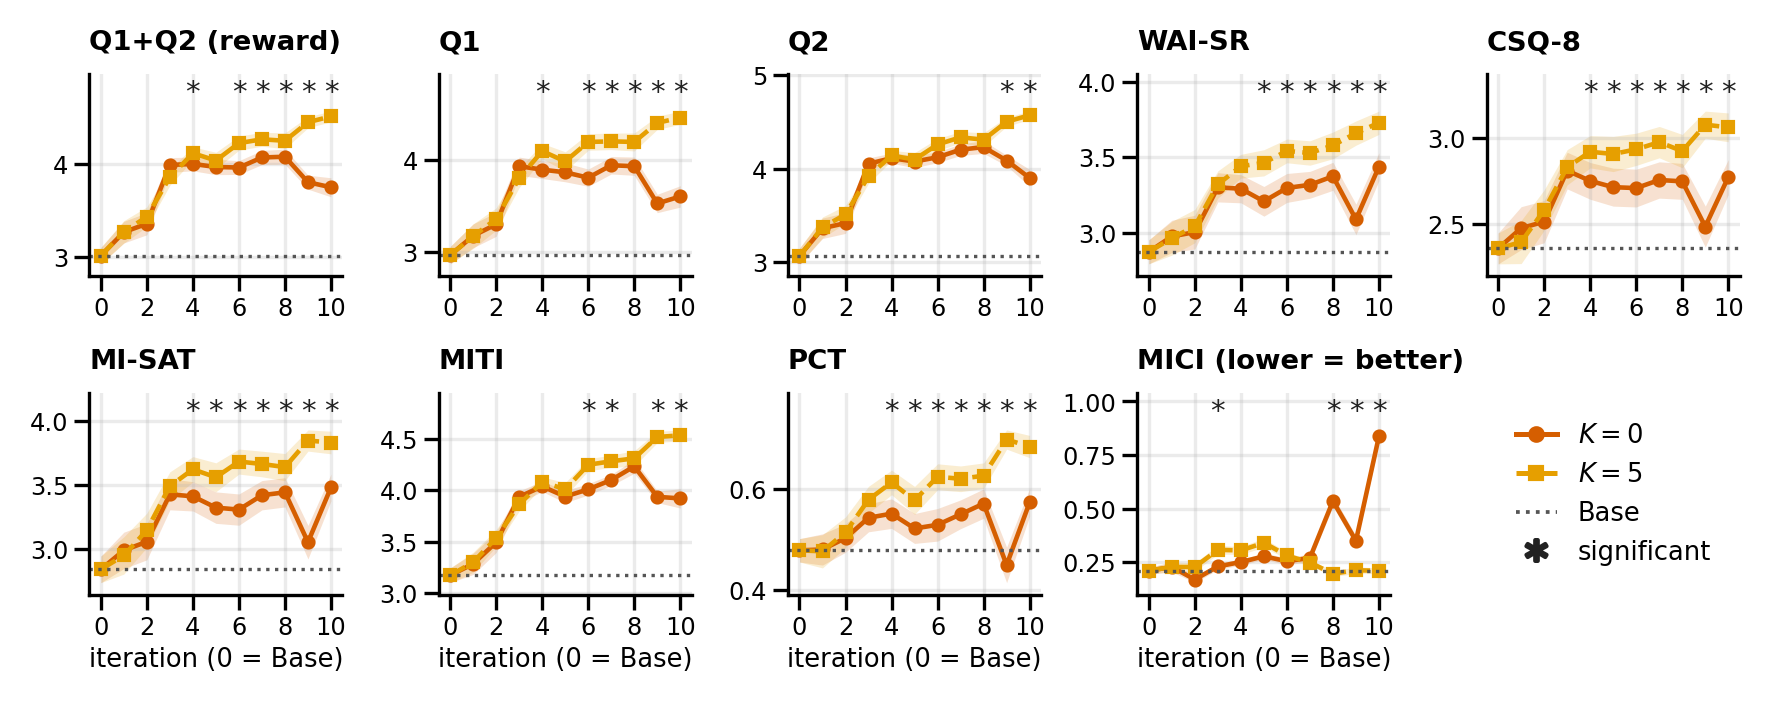
\includegraphics[width=0.94\textwidth]{figures/levels_grid_grpo_gpt-4o-mini.png}
\caption{Every instrument by iteration under the training oracle: mean $\pm$ SE over the 96
personas. Iteration 0 is the Base both runs start from (dotted line). A star marks an iteration at
which the persona-paired $\Kf$ vs.\ $\Kz$ contrast is significant; on MICI at iteration 3 it
favours $\Kz$. The held-out judge's version is Figure~\ref{fig:grid-heldout}.}
\label{fig:headline}
\end{figure*}

\begin{table*}[t]
\centering
\footnotesize
\setlength{\tabcolsep}{3.5pt}
\renewcommand{\arraystretch}{0.92}
\begin{tabular}{lrrrrrrrr}
\toprule
& \multicolumn{4}{c}{\primaryjudge\ (training oracle)} & \multicolumn{4}{c}{\heldoutjudge\ (held out)}\\
\cmidrule(lr){2-5}\cmidrule(lr){6-9}
Instrument & $\Kz$ & $\Kf$ & $\Delta$ & \dz & $\Kz$ & $\Kf$ & $\Delta$ & \dz\\
\midrule
Q1+Q2 (reward)  & $3.753$ & $\mathbf{4.517}$ & $+0.765$ & $0.905$ & $2.257$ & $\mathbf{2.873}$ & $+0.616$ & $1.030$\\
\quad Q1        & $3.606$ & $\mathbf{4.465}$ & $+0.858$ & $0.902$ & $1.867$ & $\mathbf{2.731}$ & $+0.865$ & $1.152$\\
\quad Q2        & $3.899$ & $\mathbf{4.570}$ & $+0.671$ & $0.864$ & $2.648$ & $\mathbf{3.015}$ & $+0.367$ & $0.609$\\
WAI-SR          & $3.438$ & $\mathbf{3.729}$ & $+0.291$ & $0.513$ & $2.669$ & $\mathbf{2.957}$ & $+0.288$ & $0.442$\\
CSQ-8           & $2.773$ & $\mathbf{3.062}$ & $+0.289$ & $0.482$ & $2.484$ & $\mathbf{2.935}$ & $+0.451$ & $0.678$\\
MI-SAT          & $3.479$ & $\mathbf{3.832}$ & $+0.352$ & $0.531$ & $2.825$ & $\mathbf{3.328}$ & $+0.503$ & $0.829$\\
MITI            & $3.922$ & $\mathbf{4.536}$ & $+0.615$ & $0.735$ & $2.099$ & $\mathbf{2.375}$ & $+0.276$ & $0.502$\\
PCT             & $0.574$ & $\mathbf{0.685}$ & $+0.111$ & $0.516$ & $0.612$ & $\mathbf{0.725}$ & $+0.113$ & $0.563$\\
MICI ($\downarrow$) & $0.838$ & $\mathbf{0.210}$ & $-0.627$ & $-1.862$ & $1.050$ & $\mathbf{0.628}$ & $-0.422$ & $-1.567$\\
\bottomrule
\end{tabular}
\caption{\textbf{Every instrument at iteration 10}: each run's mean over the 96 personas under each
judge (bold: the better run) and the persona-paired contrast $\Kf - \Kz$ ($n{=}96$; positive
favours $\Kf$, as does MICI's negative $\Delta$, since it is lower-is-better). \textbf{Every row is
significant at $p < .001$} (Holm across the nine rows, per judge). Levels are in each judge's own
units.}
\label{tab:endpoint}
\end{table*}

\textbf{The final policies.} At iteration 10, $\Kf$ leads on every instrument
(Table~\ref{tab:endpoint}). On the reward rubric the gap is $+0.765$ (out of 1-5 Likert scale)
($\dz\,0.905$). Measured from the Base, the $\Kf$ run gained $+1.502$ on \QQ\ and the $\Kz$ run
$+0.738$, $2.04$ times as much; measured against $\Kz$'s best checkpoint instead of its last
(iteration 8), the ratio is $1.41$. The held-out judge agrees on every row and reports the larger
standardised effect on the reward ($+0.616$, $\dz\,1.030$), with gain ratios of $2.50$ and $1.30$,
so across the two judges and both anchors the $\Kf$ gain is $1.3$ to $2.5$ times the $\Kz$ gain.

\textbf{Onset, and the $\Kz$ decline.} For the first three iterations the two runs do not differ
on \QQ\ (Figure~\ref{fig:headline}). $\Kf$ leads from iteration 4, significantly at 6 of the 10
iterations (4 and 6--10), and the other instruments follow the same course: six of the eight
separate by iteration 6, Q2 and MICI at iterations 9 and 8, and the one significant difference in
$\Kz$'s favour is MICI at iteration 3. It is not only $\Kf$ climbing: $\Kz$ peaks at iteration 8
($4.082$) and falls to $3.753$ over its last two iterations, and even against that best checkpoint
the final $\Kf$ policy leads on \QQ\ ($\dz\,0.743$, significant). The held-out judge agrees: $\Kf$
leads significantly at 7 of the 10 iterations (4--10), and against $\Kz$'s best checkpoint under
that judge (iteration 3) it still leads at $\dz\,0.386$.

\textbf{A second draw of the final policy.} Each policy is scored on one sample of 96
conversations, so we drew the final $\Kf$ policy again (96 fresh conversations from the same
adapter, personas and decoding, scored by both judges): the two draws differ by at most
$|\dz|\,0.174$ across the nine rows and both judges, none significantly, and with the second draw
the \QQ\ gap is $\dz\,0.919$ against $0.905$ (held out: $0.949$ against $1.030$). This measures how
much the scores move when the same trained model holds a new set of conversations; it says nothing
about how different a second training run would be (see Limitations).
